\newcommand{\dedx}{$\mathrm d E / \mathrm d x$ }
\chapter{Momentum estimation of slow pions with the ADC in the VXD} \label{chapter-vxd}

When looking onto the typical momentum distribution of the particles flying through the tracking detectors as show in figure \ref{fig-particles-momentum} it is clear that there is a significant amount of so called slow pions with momenta in the order of $\unit[100]{MeV}$. Slow pions play an important role for the physic analysis planned for the Belle II experiment as they are extensively used in flavor tagging decays (e.g. $\PDstar^\pm \to \PDzero \Ppipm$). Measuring the momentum of these particles leads to a better resolution in the momenta of the parent particles $\PDzero$ and $\PDstar$ which is used in separating continuous background from signal events. These slow pions get produced near the interaction point and because of their small momentum and therefore high curvature and their huge energy losses they can not be detected in the CDC tracking detector. This means they can only be measured in the VXD. Because of the small radius of the VXD and the resulting small number of independent measurement points, the momentum resolution is very poor as it can be seen in the Glückstern formula
\begin{align*}
 \frac{\sigma_{p_T}}{p_T} = \sqrt{\frac{720}{N + 4}} \sigma_x \frac{p_T \text{[GeV]}}{0.3 q B \text{[T]} L^2}
\end{align*}
where L is the length of the track in the detector and $N$ is the number of measurement points. Decreasing the magnetic field would decrease the curvature of the low momentum pions and would therefore make them detectable in the CDC also increasing the number of measurement points. But this would also make the resolution of the high momentum particles very poor. In this thesis a different approach is chosen. Together with the measured positions for each found VXD sensor hit an independent momentum estimation based on the energy loss per length of the particles in this sensor is calculated and used in the trajectory fit after the track finding. These added measurements bias the fit towards the correct momentum and can therefore help to increase the momentum resolution.

\begin{figure}
 \centering
 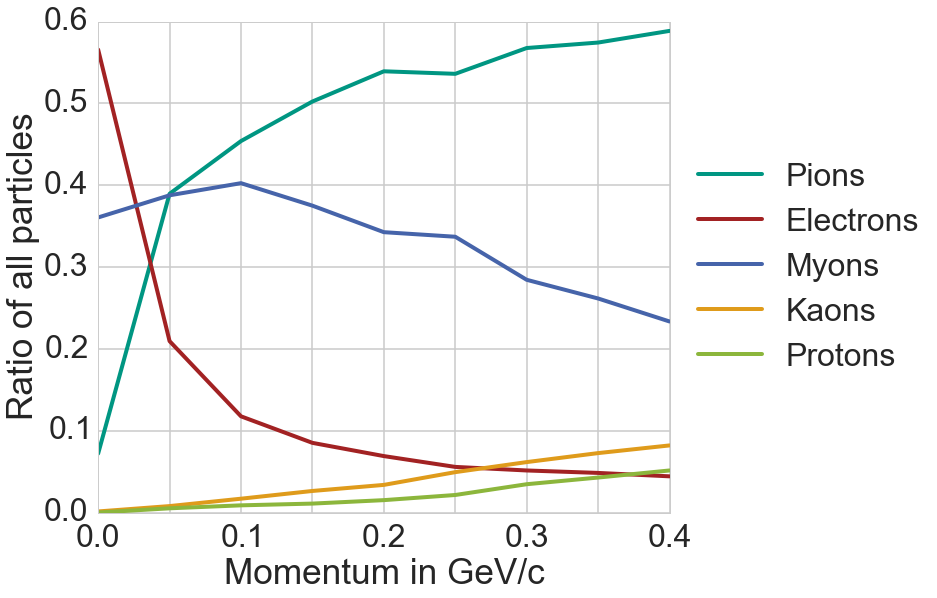
\includegraphics[width=0.8\linewidth]{figures/vxd/momentumDistribution.png}
 \caption[Momentum distribution by different particle types.]{Momentum distribution split by different particle types as generated by the simulation. As this simulation is modeled after the physical branching fractions the here shown distribution is also the expected observation in the experiment.}
 \label{fig-particles-momentum}
\end{figure}

As it was shown in previous studies \cite{robert}, the momentum resolution compared to the result of the helix fit with the positions only can be increased by using the information from the energy loss of all hits in the track together. In the quoted paper an advanced summation was used to build a mean energy loss of the slow pions which was transformed to a momentum by a predetermined formula. This momentum estimation was then compared to the one coming from the helix fit. To increase the resolution even more the two different approaches are combined in the presented algorithm.

In figure \ref{fig-dedx-over-p} the energy loss per travel length in the VXD sensors for low momentum pions is shown. How these numbers are calculated is described in the next sections. As it can be seen the \dedx increases with falling momentum of the particles. This relation can be also seen in the already quoted Bethe formula \ref{form-bethe} in chapter \ref{chapter-ex} which can be reduced to 
\begin{align}
 -\left \langle \dd{E}{x} \right\rangle \approx \frac{4 \pi n z^2}{m_e v^2} \left( \frac{e^2}{4 \pi \varepsilon_0} \right)^2 \ln \left( \frac{2 m_e v^2}{I} \right) \label{form-bethe-simpl}
\end{align}
for small particle energies. The equation can be used to calculate the momentum using the energy loss per travel length. But as this formula describes the averaged energy loss it is only correct for a small number of cases. The variance in the energy loss is distributed according to a landau distribution which is described later in more detail. This deviation from the Bethe formula decreases the momentum resolution of the estimation based on the energy loss.

\begin{figure}
 \centering
 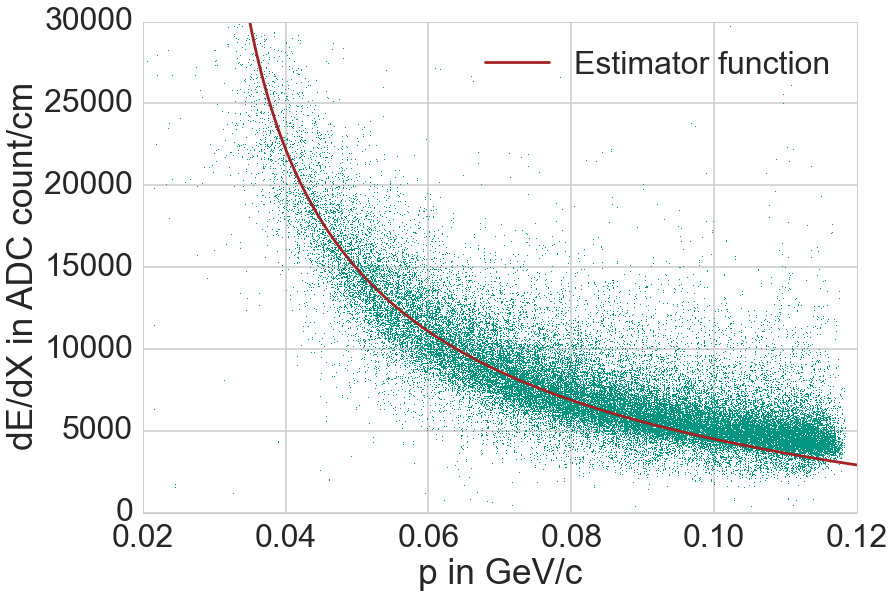
\includegraphics[width=0.8\linewidth]{figures/vxd/dedxWithEstimator.png}
 \caption[\dedx information of the VXD clusters.]{\dedx information of the VXD clusters of approximately 100000 pions in the momentum range from 50 to 120 MeV. The averaged energy loss can be described by the Bethe formula. The distribution of energy losses for a given momentum is distributed according to a landau distribution which is described later in more detail. To transform the \dedx value to a momentum the red estimator curve is used later.}
 \label{fig-dedx-over-p}
\end{figure}


\section{Prestudies on the distribution of dE/dX in the VXD}

For the following studies an event sample of slow pions in the momentum range between $\unit[50]{MeV}$ and $\unit[120]{MeV}$ is used. It is simulated using the particle gun with 10 particles per event evenly distributed among the momentum range and between the two charge modes. The sample is split into different event samples for testing and training. The standalone VXD track finder or the MC track finder for reference is used to create tracks out of the simulated VXD hits. As the finding efficiency of the standalone VXD track finder depends heavily on the momenta of the particles, the distribution of the found tracks is not flat any more as it can be seen in figure \ref{fig-vxd-finding-efficiency}. A typical event display can be seen in picture \ref{fig-vxd-event-display}.

\begin{figure}
 \centering
 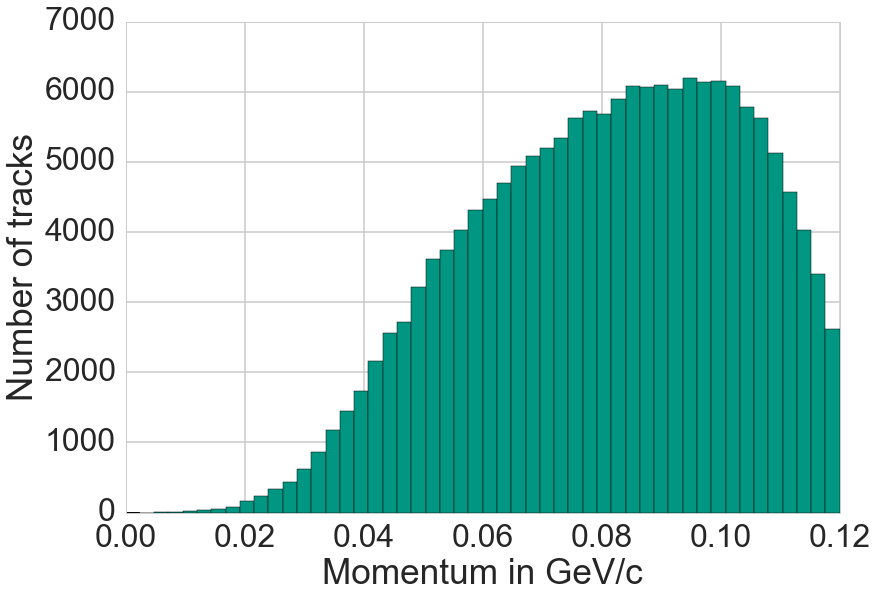
\includegraphics[width=0.48\linewidth]{figures/vxd/finding_efficiency.png}
 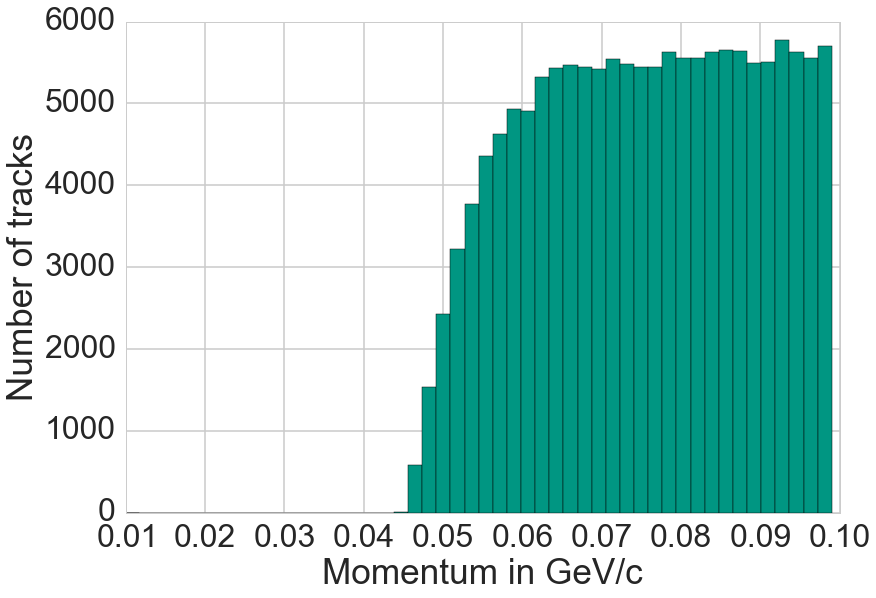
\includegraphics[width=0.48\linewidth]{figures/vxd/finding_efficiency_mc.png}
 \todo{why is there a drop?}
 \caption[Momentum distribution of the found and simulated pions.]{Momentum distribution of the simulated pions as found by the VXD track finder (left) and the MC track finder (which has the simulated truth information, right). The finding efficiency decreases with lower momenta as the number of hits in the VXD is lower for slow pions and the energy loss is stronger. The MC track finder has also not a flat distribution of momenta as it only uses those particles for tracks which have at least 3 hits in the VXD detector.}
 \label{fig-vxd-finding-efficiency}
\end{figure}

\begin{figure}
 \centering
 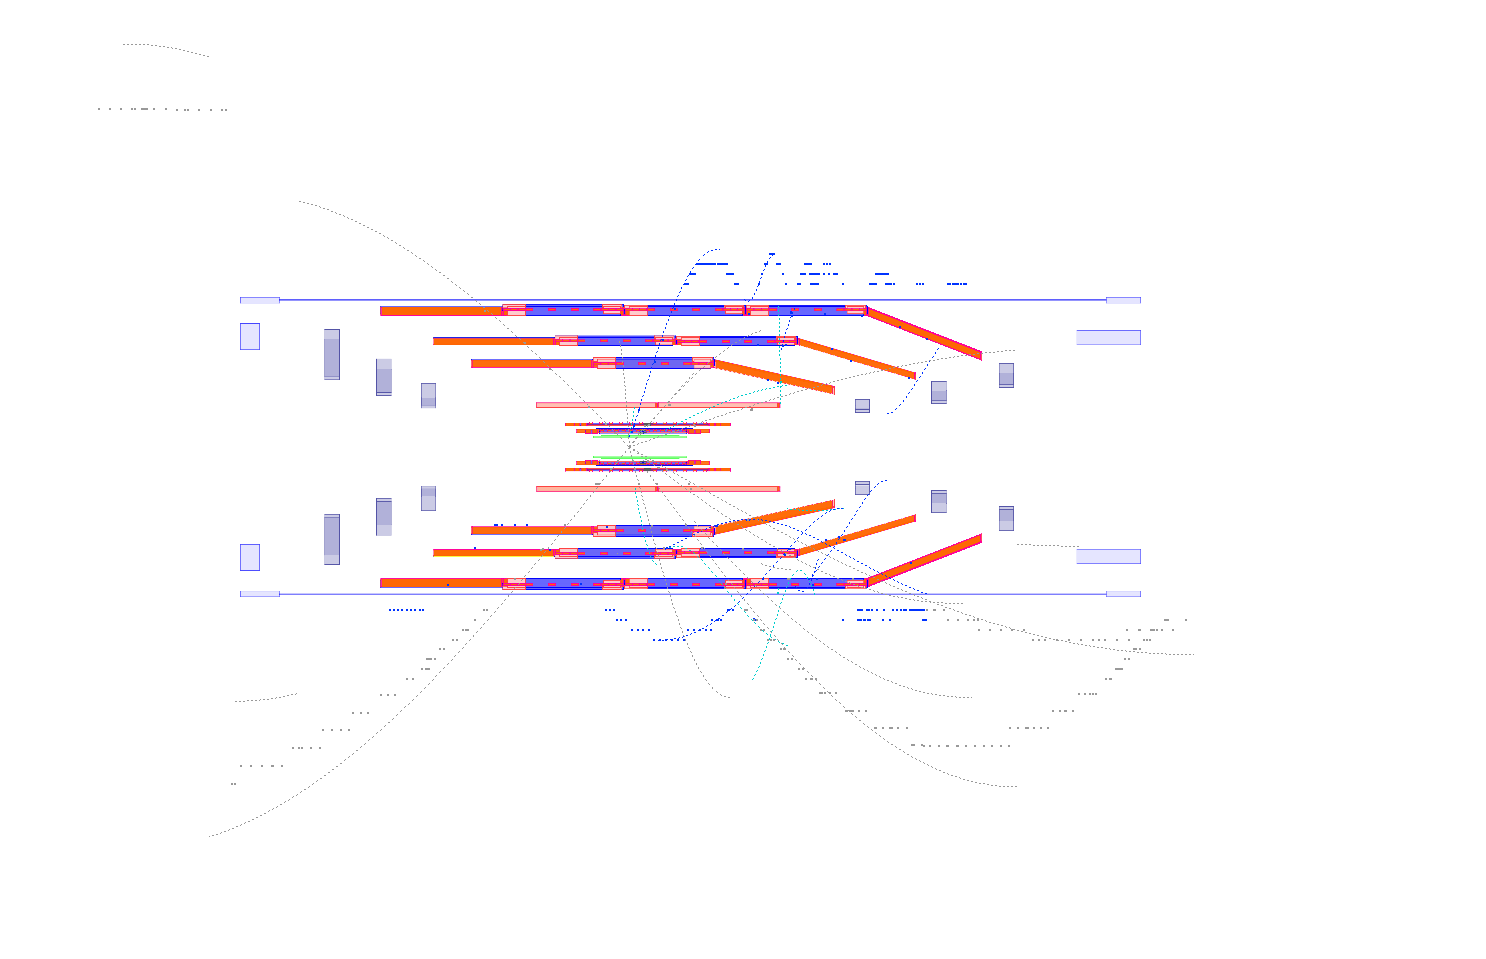
\includegraphics[width=0.8\linewidth]{figures/vxd/event_display.png}
 \caption[Typical event display of slow pions.]{Typical event display of one event used for analyzing the momentum estimation for the fitting procedure in the helix fit. The blue box depicts the inner wall of the CDC. As it can be seen, most of the particles do not reach into the drift chamber and can only be detected with the VXD sensors.}
 \label{fig-vxd-event-display}
\end{figure}

Before calculating the function to transform the \dedx value to a momentum estimation and using this information in the helix fit some prestudies are performed to check for the consistency of the input data. They are shown here for reference too.

For calculating the path length used in \dedx the correct position of the hit and the sensor information is needed. This information is provided by the clusters used in the track finder. Its results can be seen in figure \ref{fig-cluster-position} where the distance to the beam pipe over the z position is shown for some SVD hits. This position is later used to calculate the path length of the tracks in the sensor region.

\begin{figure}
 \centering
 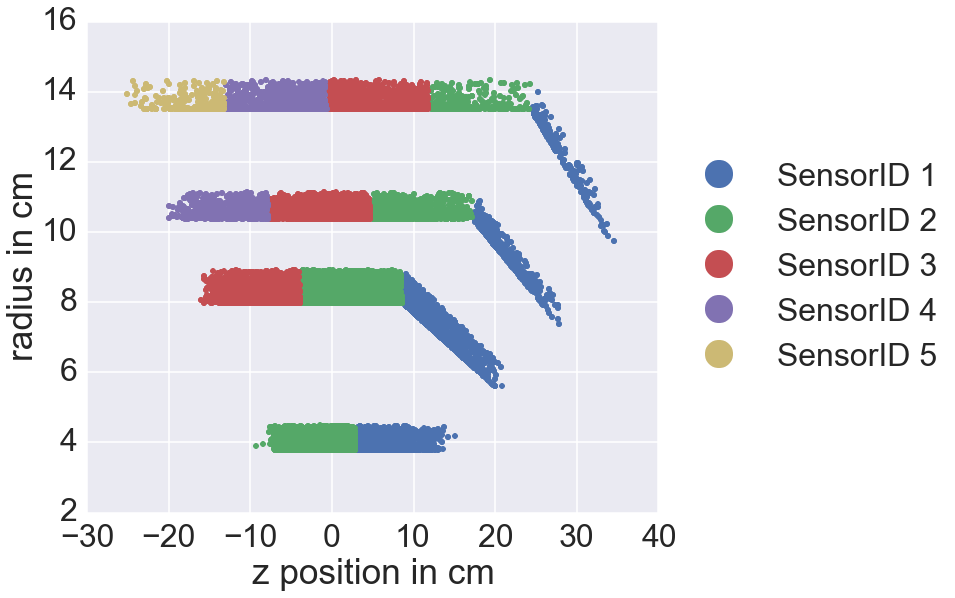
\includegraphics[width=0.8\linewidth]{figures/vxd/cluster_positions.png}
 \caption[Picture showing the simulated hit information.]{Picture showing the simulated hit information of the first 1000 clusters in the event sample. The color code separates between the sensor ID property of the clusters.}
 \label{fig-cluster-position}
\end{figure}

Instead of using the deposited charge in every sensor directly the ADC count value of every sensor is used. This ADC count comes directly from the digitalization process and does therefore not rely on any calibration process. As it is directly proportional to the deposited energy and the parameters of the transformation function from \dedx to the momentum have to be determined by a fit in either way, the ADC count is used as a measure for the energy deposition. Picture \ref{fig-adc-count} shows the the \dedx value calculated with this ADC count for the two different detectors SVD and PXD. As it can be seen, the calibration coefficients to the correct deposited energy are different for the two detectors and therefore the two distributions are not superimposable. To cope with this fact the ADC counts coming from the PXD sensors get multiplied by a factor of 0.565868 which was calculated on data. The resulting distribution is shown in the right subplot of figure \ref{fig-adc-count}. This calibration is mainly done to be able to treat both hit types in the same manner later. 

\begin{figure}
  \centering
 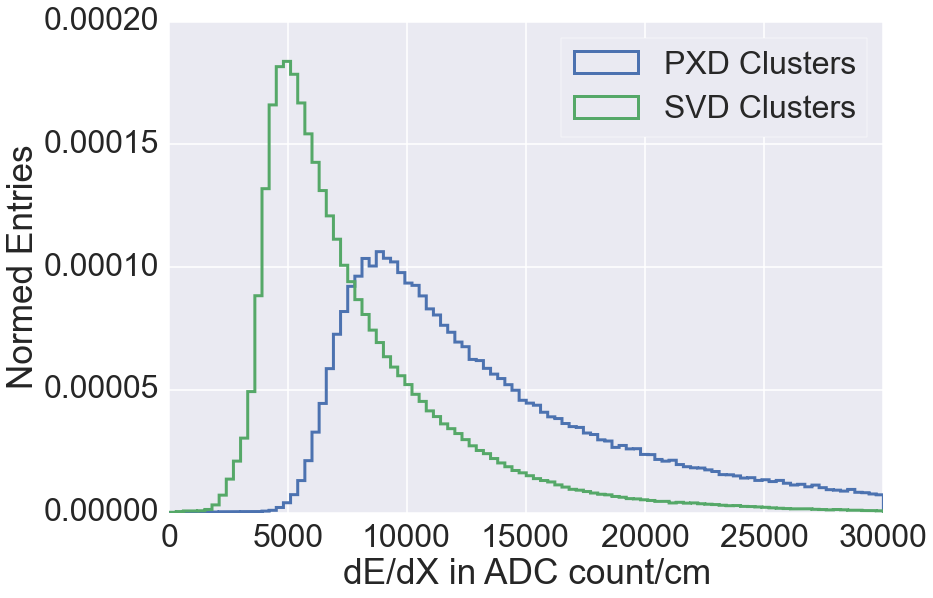
\includegraphics[width=0.48\linewidth]{figures/vxd/dEdXUncalibrated.png}
 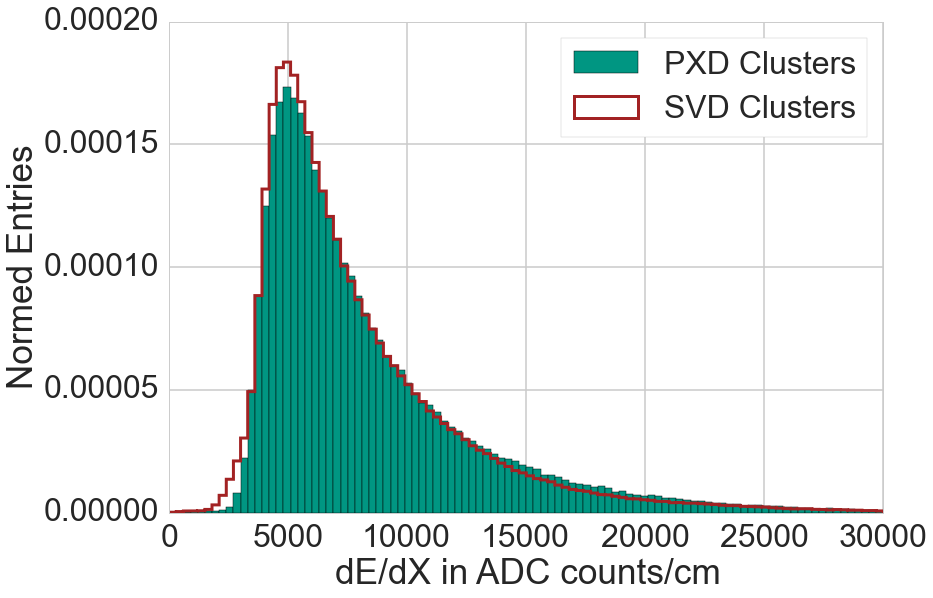
\includegraphics[width=0.48\linewidth]{figures/vxd/dEdXCalibrated.png}
 \caption[Distributions of the uncalibrated and the calibrated ADC counts.]{Distributions of the uncalibrated (left) and the calibrated (right) ADC counts of the PXD and SVD hits. Only clusters found by the VXD track finder are shown here.}
 \label{fig-adc-count}
\end{figure}

\subsection{Calculation of the path length in the clusters} \label{subsection-calc}
The \dedx value in every cluster can be calculated using the calibrated charge as described above and the length of the path the particle travels in the sensor region. There are five ways to calculate this path length. All of them are implemented in the code basis.
\begin{zlist}
 \item Using the correct (simulated) MC trajectory information of the tracks at the position of the clusters, \label{list-mc}
 \item Using the current trajectory parameters while fitting,
 \item Using the related MC trajectory at the origin,
 \item Using the trajectory parameters estimated by the track finder without MC truth information,
 \item Using the thickness of the cluster.
\end{zlist}

The different possibilities are ordered by their anticipated correctness. The two MC modes are only implemented for reference as they can obviously not be used in the later detector measurement. How the current trajectory parameters are deduced in the fit is described later.

Besides the last possibilities all modes rely on calculating the path length of a trajectory using their helix parameters. As the calculated path lengths are very small, this is done without taking into account energy loss or material effects. The procedure is as follows:
\begin{zlist}
 \item Take the position of the cluster hit (the point where the trajectory enters the VXD sensor) and calculate the distance to the beam line. This is called the inner radius of the cluster.
 \item Add the sensor thickness to this radius to gain an estimation of the outer radius of the sensor.
 \item Calculate the arc length between these two radii and from this arc length the distance between the two penetration points of the helix through the sensor using trigonometrical relations.
\end{zlist}

This procedure is correct for most of the time but fails in some rare cases. Some examples are shown in figure \ref{fig-errors-in-path-length}. As it can be seen in the pictures, errors in the calculation occur mainly for particles which have their apogee\footnote{The apogee is the opposite to the perigee - the point on the helical trajectory the most far away from the interaction point} in the sensors. As the VXD sensors have only a very thin thickness the probability for such particles is very rare. Therefore these cases do not bias the momentum measurement much. Also as the calculation error can only occur in the most outer sensor touched by the particles all other sensors give correct momentum estimations. A short preliminary study shows that only about 0.4 \% of the particles are affected.

\begin{figure}
  \centering
  \raisebox{-0.5\height}{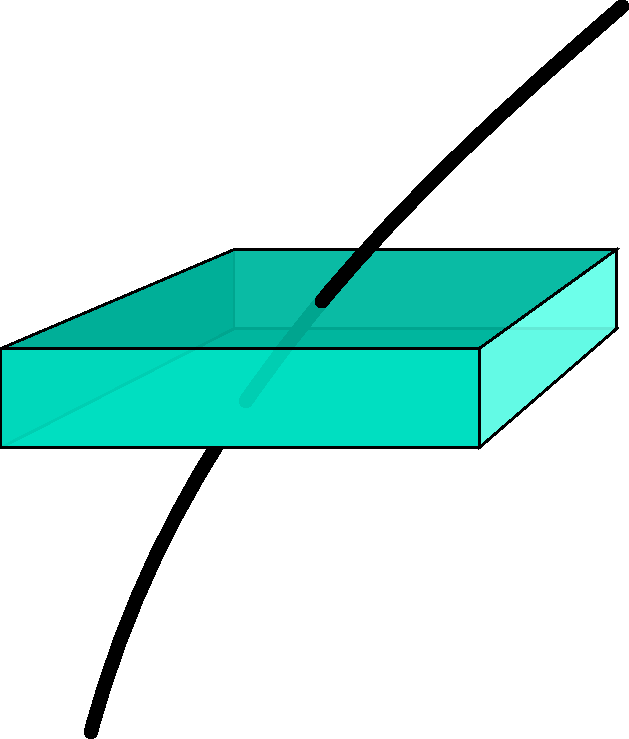
\includegraphics[scale=0.3]{figures/vxd/pathlength1.pdf}}
  \hspace*{1.5cm}
  \raisebox{-0.65\height}{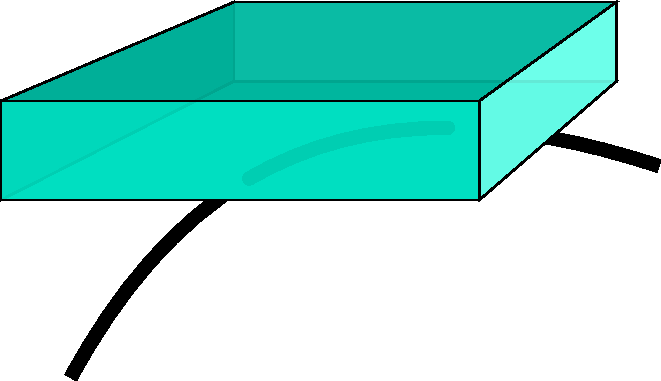
\includegraphics[scale=0.3]{figures/vxd/pathlength3.pdf}}
  \hspace*{0.5cm}
  \raisebox{-0.5\height}{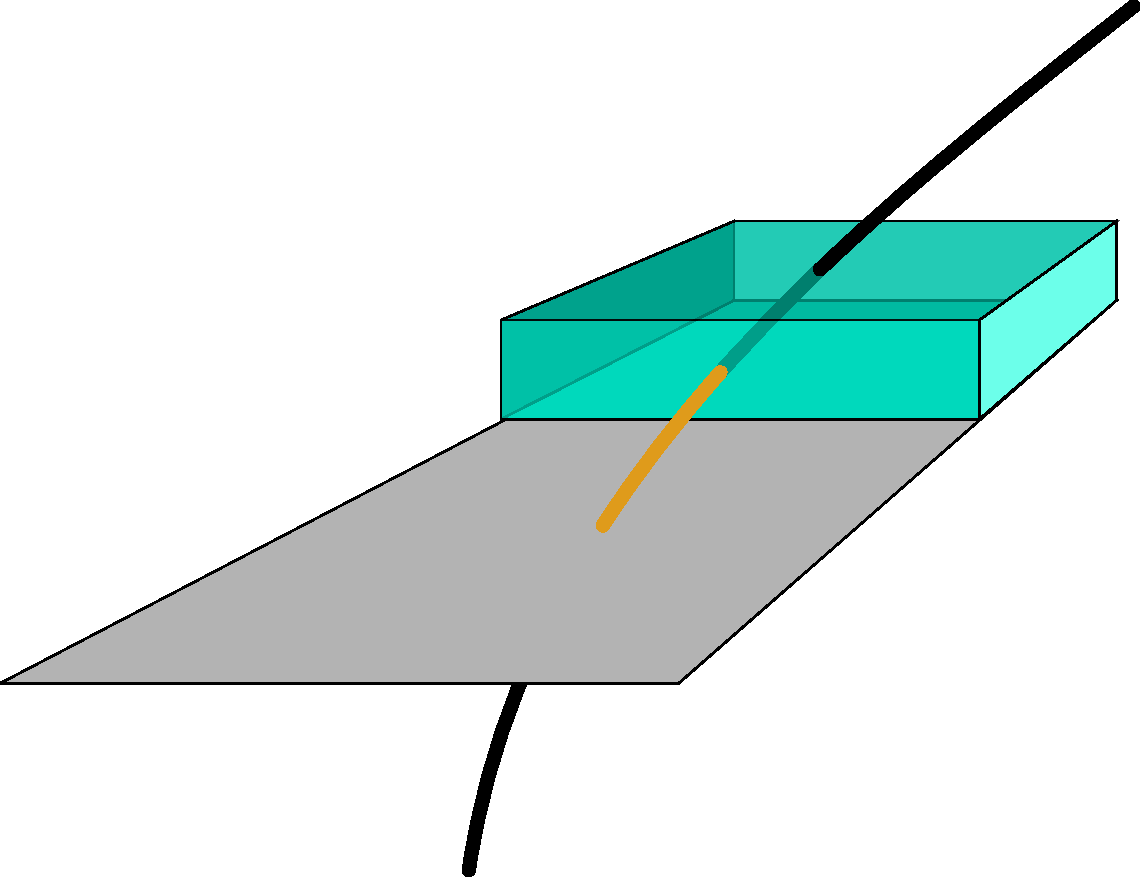
\includegraphics[scale=0.3]{figures/vxd/pathlength4b.pdf}}
  \caption[Exemplary cases of path length calculations.]{Exemplary cases of path length calculations. The algorithm fails in the second and last case. In the second case it returns the width or the length of the sensor instead. In the last case it wrongly adds the orange part of the path length to the correct one. Because of the geometrical dimensions of the sensors these two cases are very rare.}
  \label{fig-errors-in-path-length}
\end{figure}

In figure \ref{fig-pathlengths} the distribution of the path lengths from the simulated MC truth values is shown. As most of the particles go more or less straight through the sensors, there are two peaks in the distribution - one for each hit type as the two types PXD and SVD have a different thickness. Deviations from the thickness come from curling particles. The fact that there are only few tracks with very high deviations from the thickness values verifies the claim that the helix calculation is wrong only for very rare cases.

The second subplot shows the distribution of the residuum of the other four path length calculations to these reference values as a violin plot.

As it can be seen... \todo{Beschreibung!}

\begin{figure}
 \centering
 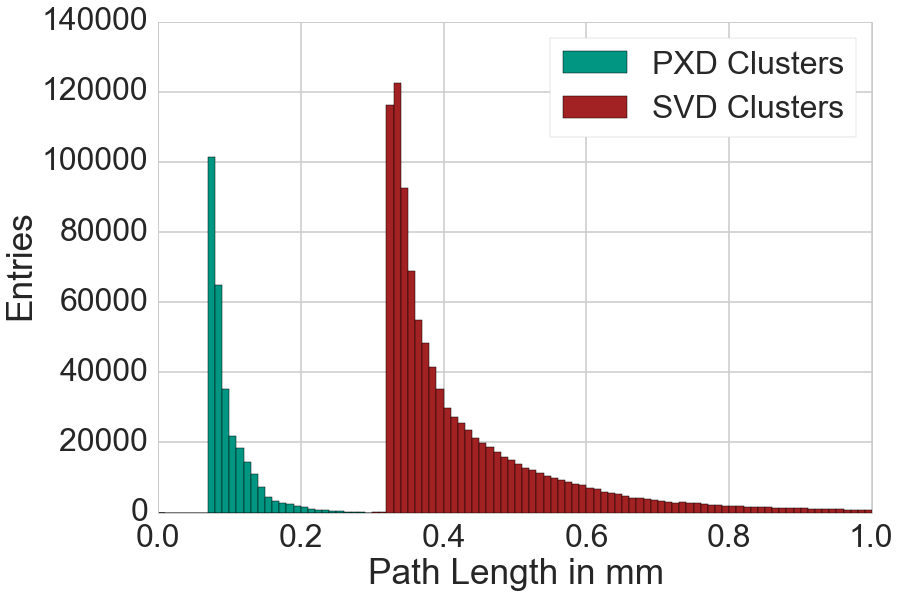
\includegraphics[width=0.7\linewidth]{figures/vxd/pathLengths.png}
%   \includegraphics[width=0.7\linewidth]{figures/vxd/pathLengthsDifferentCalculations.png}
 \todo{picture}
 \caption[Path length distribution for the two sensor types.]{The plot shows the path length distribution for the two sensor types as a result of the simulation. This distribution is used for reference in the right plot which shows the residuum distribution of the other path length calculation modes.}
 \label{fig-pathlengths}
\end{figure}

\subsection{Transformation function from dE/dX to momentum} \label{subsection-transform}

For calculating a momentum estimation from the \dedx value the inverted function of equation \ref{form-bethe-simpl} is needed which can not be calculated analytically. Therefore a much easier model function
\begin{align}
 p(\mathrm{d}E/\mathrm{d} x) = \frac{a}{(\mathrm{d}E/\mathrm{d} x - b)^2} + c \cdot \mathrm{d}E/\mathrm{d} x + d \label{form-model}
\end{align}
with the free parameters $a, b, c$ and $d$ is fitted to the $\mathrm d E / \mathrm d x$-momentum-values where \dedx is calculated with path lengths from mode (\ref{list-mc}) and the momentum is taken from the MC simulation at this cluster (so including energy loss by material effects).

The fitting parameters can not be determined by fitting the model function to the whole distribution at once as shown for example in figure \ref{fig-dedx-over-p}. The reason is that because of the landau distributed energy loss the number of outliers is too high and causes the fit to fail. An example of the landau distribution showing the large amount of outliers deviating from the mean energy loss is shown in picture \ref{fig-landau}. This is why a reduce approach is chosen here: First the $\mathrm d E / \mathrm d x$-range is split into several small bins. In each of them the momentum distribution is build. This distribution is then fitted with a landau or a normal distribution. Mathematically, the momentum distribution in these $\mathrm d E / \mathrm d x$-bins is neither distributed according to a landau nor a normal distribution but the correct form can not be calculated analytically and these two distributions describe the data best.\footnote{The correct form of the distribution can be calculated by integrating over parts of the landau distribution folded with the inverted Bethe-equation, which is not analytically solvable.} The resulting parameters of the distributions (the mean of the gauß or the location parameter of the landau distribution\cite{landau}) are then used for fitting the model function (\ref{form-model}). The whole process can be seen in figure \ref{fig-fit-bins}.

\begin{figure}
  \centering
  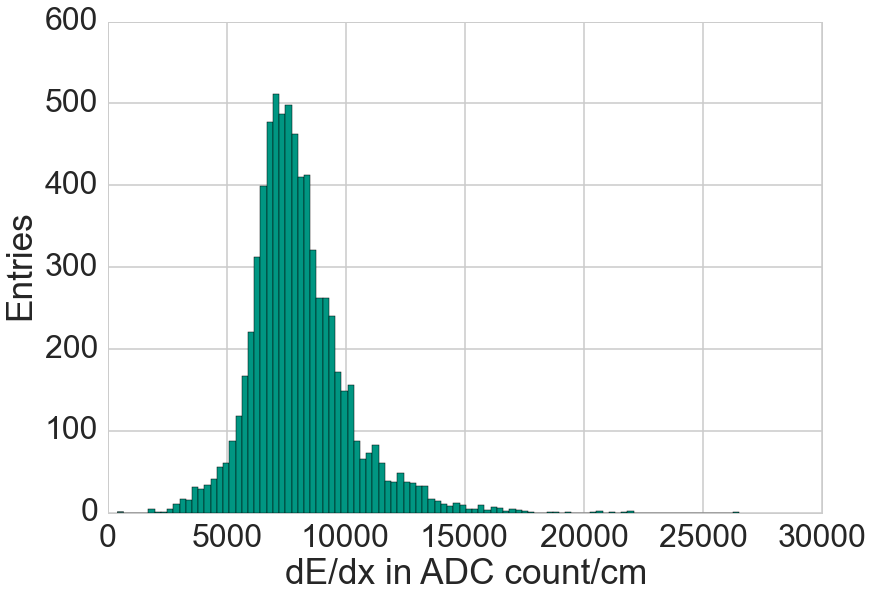
\includegraphics[width=0.7\linewidth]{figures/vxd/landau.png}
  \caption[Energy loss of particles in a sharp momentum range near of 70 MeV.]{Energy loss of particles in a sharp momentum range near of $\unit[70]{MeV}$. The distribution spreads over a large area in the \dedx space which causes the fit of the momentum estimation function to the raw data to fail.}
  \label{fig-landau}
\end{figure}

\begin{figure}
  \centering
  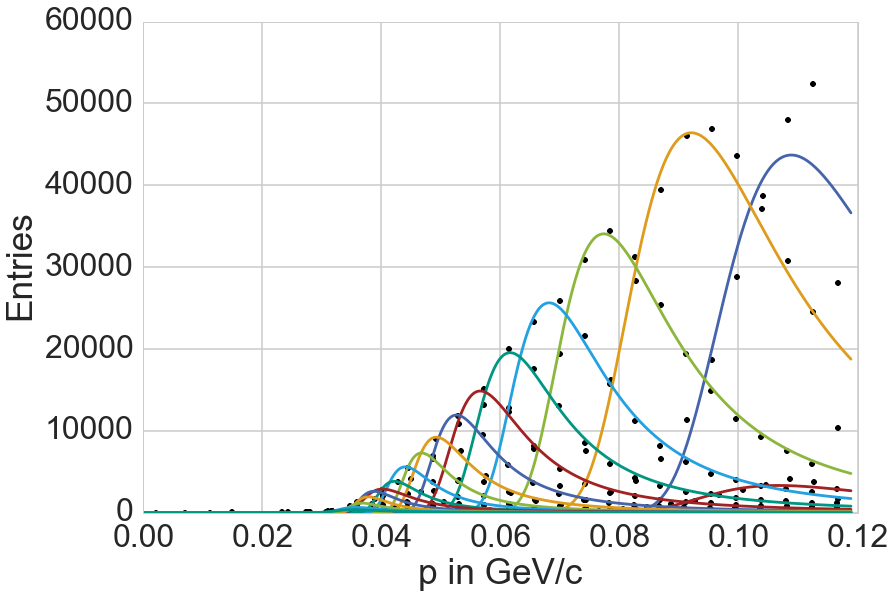
\includegraphics[width=0.48\linewidth]{figures/vxd/fitLandau1.png}
  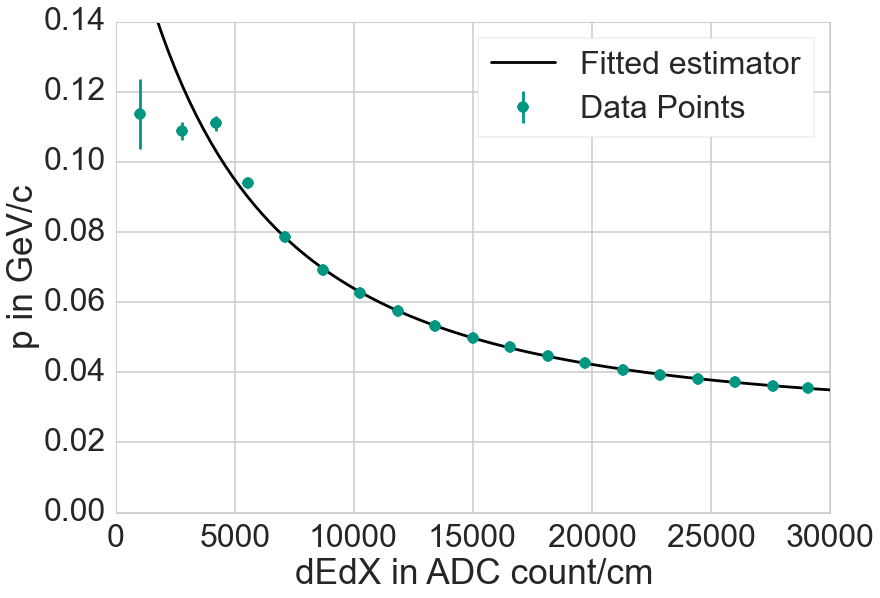
\includegraphics[width=0.48\linewidth]{figures/vxd/fitLandau2.png}
  \caption[The process of obtaining the estimator function $p(\mathrm d E/\mathrm d x)$.]{The process of obtaining the estimator function $p(\mathrm d E/\mathrm d x)$. The left picture shows the p-distributions for 15 \dedx bins. Each of the distributions get fitted by a landau distribution. The right plot shows the location parameter of these fitted landau distributions. These values are then used to fit the model in equation (\ref{form-model}).}
  \label{fig-fit-bins}
\end{figure}

For the incorporation of the gained momentum estimation into the helix fit of genfit, not the momentum value directly but $q/p$ is needed. This is why in the following the residuum of $p^{-1}$ instead of $p$ is presented.

In the two subplots of figure \ref{fig-divp-residuum} the median and the interquartile range of the residuum of the estimated to the MC momentum is shown. As both fit functions (gauß and landau) lead to quite large shifts in the median indicating a biased momentum estimation a correction procedure is introduced: a cubic polynomial is fitted to the median values which is later subtracted from the momentum estimation. These corrected estimators are also shown in the figure. They do reduce the median of the residuum but increase the IQR in turn.

\begin{figure}
  \centering
   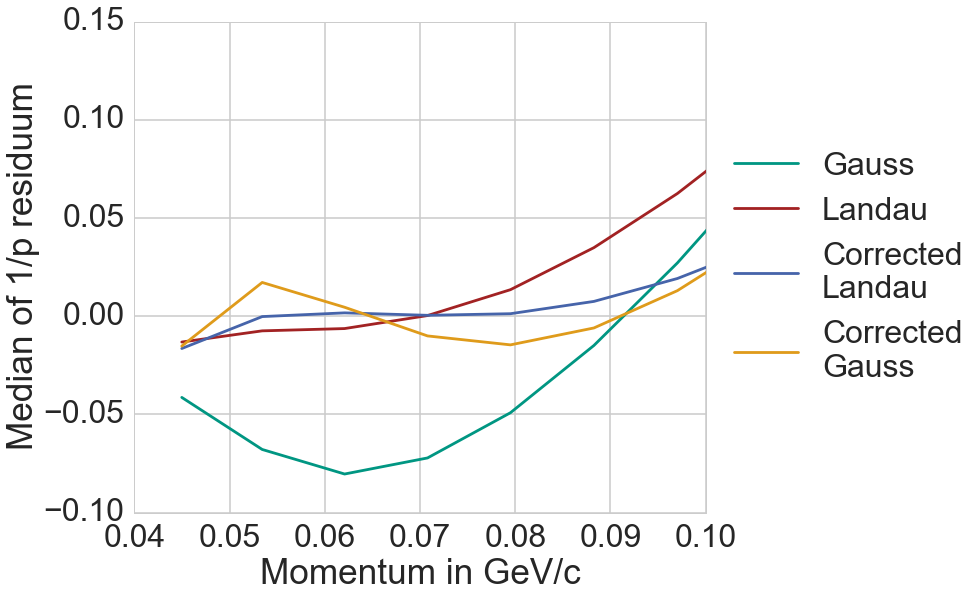
\includegraphics[width=0.47\linewidth]{figures/vxd/divPMedian.png}
   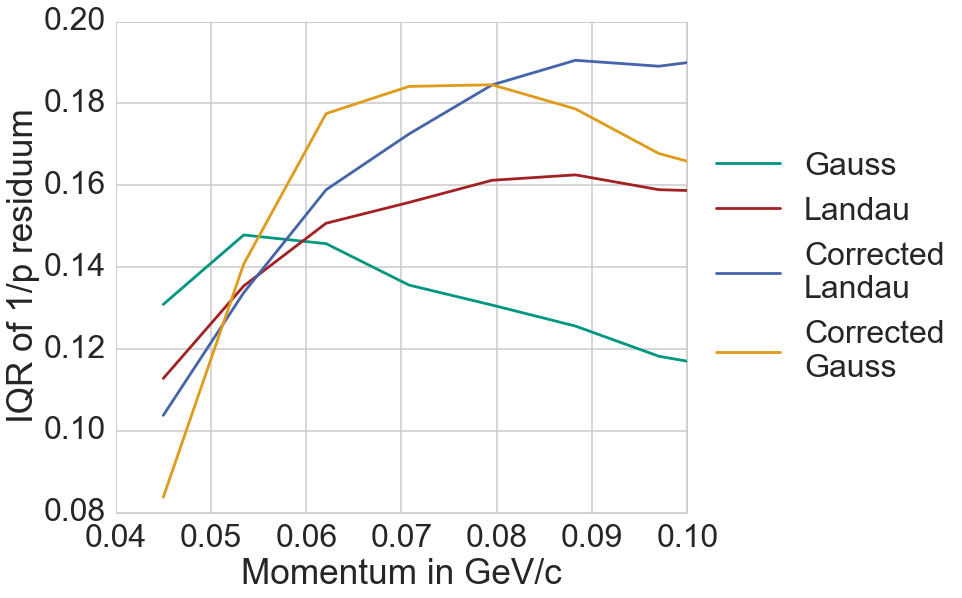
\includegraphics[width=0.47\linewidth]{figures/vxd/divPIQR.png}
  \caption[Median and IQR of $1/p$.]{The median (left) and the interquartile range (right) of the residuum between $1/p$ calculated with the estimator function and the MC information over the MC momentum. For all path length calculations the MC information at the hit is used. Together with the two fit functions landau and gauß also the median-corrected estimators (as described in the text) are shown.}
  \label{fig-divp-residuum}
\end{figure}


Besides the here presented two methods to gain the estimator function $p(\mathrm dE/\mathrm dx)$, also other fit models instead of equation \ref{form-model}, other fit functions instead of landau and gauß and totally different methods like a boosted decision tree for regressions were tested. As all of these methods show worse results, they are not presented here. They can be easily compared to the mentioned results by using the IPython notebooks written by the author of this thesis.

\section{Incorporation in the helix fit}

Before describing the results of the momentum resolution with and without the new momentum estimation, the incorporation of this new measurement type is described shortly. For this, the measurement model used in genfit is summarized here briefly. More information can be found elsewhere \cite{genfit}.

The idea of the genfit package as a generalized track fitting package is to not rely on a certain detector configuration but rather threat the measured hits in a general form. For this, every hit is transformed into an derived class of an \texttt{AbsMeasurement}. This general measurement can hold up to five general coordinate measurements, which are two local coordinates $u$ and $v$, two local direction measurements $u'$ and $v'$ and an measurement for $q/p$. The measurement stores also the errors and covariances of these measurements and a generalized plane one which the measurements and the local coordinates are defined. The user does not have to provide all coordinate measurement on every \texttt{AbsMeasurement}. This general scheme makes it possible to incorporate all different results of the measuring detectors, e.g. VXD hits (which define a plane as the sensor plane and give one coordinate measurement of $u$ or $v$ for each strip in the case of SVD hits and both coordinates for PXD hits) or CDC wire hits (where the definition of a plane is more difficult to choose leading to a redefinition of the plane in every fit iteration). As the real detector measurements are uncoupled from the fitting algorithm, the implemented fitters do not have to be adopted to cope with different measurements.

To include the momentum estimation based on the \dedx value into the fit also, one has therefore to include another \texttt{AbsMeasurement} into the tracks for each VXD hit which is only filled with the $q/p$-coordinate and has the same plane as the positional measurement for this VXD hit. Another possibility would be to include this coordinate also in the already created positional measurements (by filling the two local positions $u$ and $v$ and the $q/p$ coordinate also). The downside of this approach is that the DAF described in chapter \ref{chapter-theory} is then only able to downweight the whole measurement with the positional and the momentum coordinates and not the single measurement types only.

\subsection{Code basis for the fitting procedure}

In parallel to adding the momentum estimation to the VXD hits - but for other reasons also - the whole fitting framework in basf2 was rewritten. The former \texttt{genfit::Track} and the \texttt{genfit::TrackCand} where merged into a \texttt{RecoTrack} based on the \texttt{genfit::Track} which suits better to the StoreArray-scheme of the framework. Together with the new \texttt{RecoTrack} also other modules for fitting had to be written. The former \texttt{Genfitter} module was split up into smaller modules, each handling a single task. In the following, only the \texttt{MeasurementCreatorModule} will be described. More information on the \texttt{RecoTrack} and the other modules can be found in chapter \ref{chapter-addon}.

The task of this module is to create the measurements for each hit added to the \texttt{RecoTrack} by the track finding algorithms. The measurements can then be used by the track fitting routine. The \texttt{MeasurementCreatorModule} does so by calling configurable \texttt{MeasurementCreator} objects on all hits which can create a measurement out of the hit and the \texttt{RecoTrack}. There are preconfigured \texttt{MeasurementCreator} classes for turning the found hits into normal positional measurements like it was done before by the \texttt{GenfitterModule}. To handle the configuration of these \texttt{MeasurementCreator} objects in an easier way, the design pattern of factories was used in the module. Each type of \texttt{MeasurementCreator} objects (for looping over SVD, PXD or CDC hits found by the track finder or for no underlaying track finder hit at all) has an \texttt{MeasurementCreatorFactory}. These factories handle the configuration and initialization of the \texttt{MeasurementCreator} objects which in turn create measurements and add them to the \texttt{RecoTrack}. The configuration of the factories can be done via dictionaries passed as module parameters in the steering files. The whole process is shown in figure \ref{fig-measurement-creator}.

\begin{figure}
  \centering
  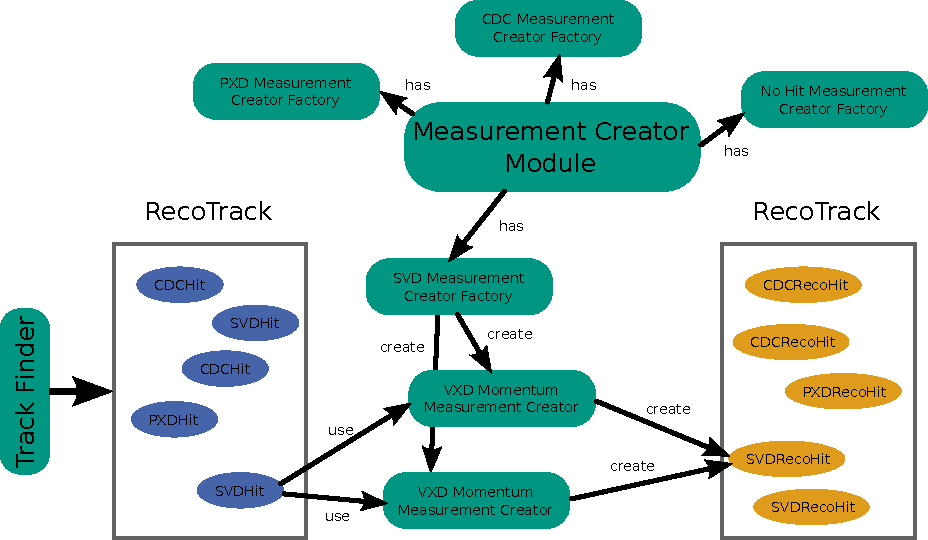
\includegraphics[width=\linewidth]{figures/vxd/measurementCreator.pdf}
  \caption[Diagram showing the creation of measurements.]{Diagram showing the creation of measurements in the \texttt{MeasurementCreatorModule} as described in the text. Each \texttt{RecoTrack} includes PXD, SVD and CDC hits (blue) added by the track finder algorithms which must be transformed into \texttt{AbsMeasurement} objects (orange) to be handled by the track fitting routine later. These measurements can include positional, directional and/or $q/p$ coordinate values with their errors.}
  \label{fig-measurement-creator}
\end{figure}

The momentum estimation of the VXD hits is included into the fit as another measurement - created also by a \texttt{MeasurementCreator} object. The measurements are created before the track fit but get called for their parameters in ever fitting iteration right before the fit uses the coordinates in the measurement. This fact can be used to calculate the plane (as used in the CDC hits) or the coordinates just before using them. Therefore it is possible to use the fitted state right in front of the hit to calculate the path length as described in subsection \ref{subsection-calc}. Together with the estimation for $q/p$ also the error on this coordinate has to be included into the \texttt{AbsMeasurement}. This error can be calculated using the MC momentum used for calculating the estimator function and comparing this to the estimator function result. The error is fixed to 0.3 in the moment, but can in principle be also calculated for every measurement independently.

\subsection{Results for the resolution after track fitting}

The above described estimation is included as a \texttt{MeasurementCreator} for SVD and PXD hits and the pion tracks in the momentum range of 50 - 100 MeV are fitted using the Kalman filter. Then the momentum calculated in the fit is compared to the one used in the MC simulation. To show the resolution in an easier way, the median and the interquartile range for the residuum is calculated. They can be seen in figure \ref{fig-results-fit} for both fit functions landau and gauß (with their median-corrected estimators also) and for the different path length calculations in figure \ref{fig-results-fit2}.

\begin{figure}
  \centering
%   \includegraphics[width=0.48\linewidth]{figures/vxd/fitMedian.png}
%   \includegraphics[width=0.48\linewidth]{figures/vxd/fitIQR.pdf}
%   \includegraphics[width=0.48\linewidth]{figures/vxd/fitCount.pdf}
  \todo{picture}
  \caption[Residuum of the momentum estimation for different fit functions.]{Figure showing the median (left) and the interquartile range (right) for the residuum between the MC momentum and the momentum coming from the helix fit with or without the momentum estimation based on the energy loss information. The two different fit functions landau and norm (like described in subsection \ref{subsection-transform}) are both shown here. The third plots shows the number of successful fits divided by the number of found tracks.}
  \label{fig-results-fit}
\end{figure}


\begin{figure}
  \centering
  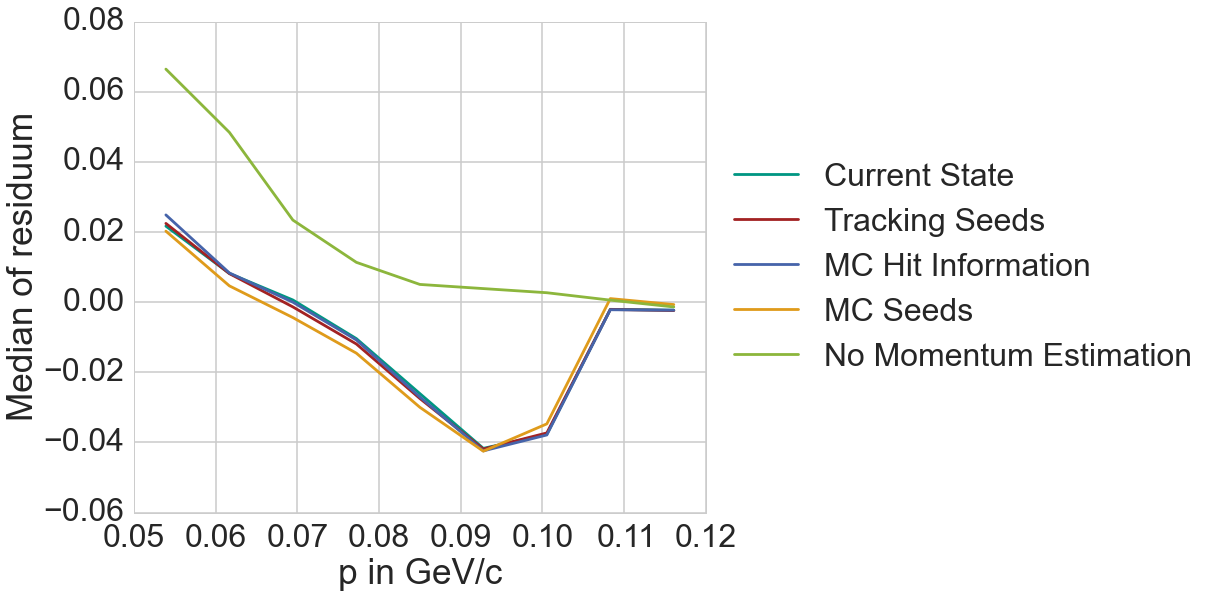
\includegraphics[width=0.48\linewidth]{figures/vxd/landauKalman0_3Median.png}
  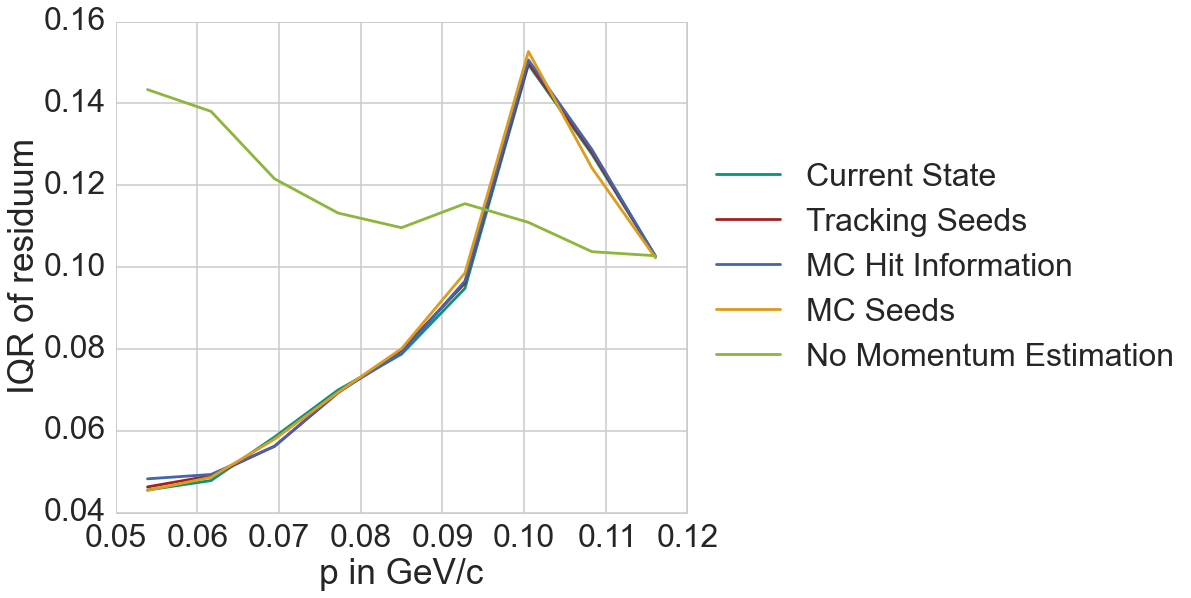
\includegraphics[width=0.48\linewidth]{figures/vxd/landauKalman0_3IQR.png}
  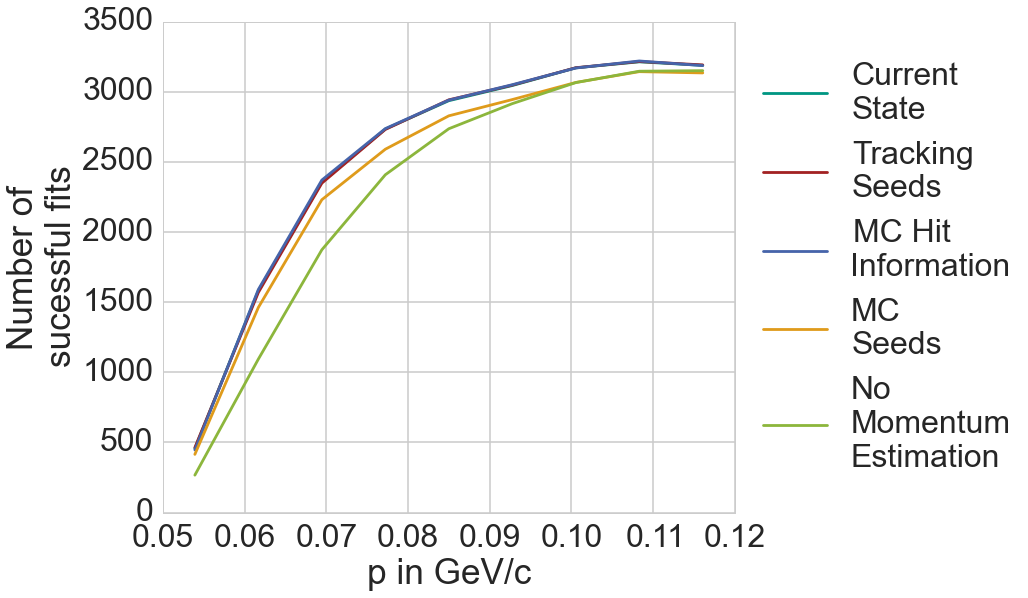
\includegraphics[width=0.48\linewidth]{figures/vxd/landauKalman0_3Count.png}
  \caption[Residuum of the momentum estimation for different path length calculations.]{Figure showing also the median (left) and the interquartile range (right) of the residuum and the ratio of successful fits as in figure \ref{fig-results-fit}. This time the different path length calculations are shown for the case of using a landau distribution for fitting the \dedx values.}
  \label{fig-results-fit2}
\end{figure}

As it can be seen in the result figures, the incorporation of the VXD momentum estimation into the helix fit can increase the resolution of the momentum quite drastically for low momentum tracks while also increasing the number of successful fits. As the landau seems to perform slightly better than the gauß fitted estimator function, these values are used in the following. Although the median-corrected functions should theoretically behave better, the resolution could not be increased. This may come from the worsen IQR of the corrected estimators as seen in figure \ref{fig-divp-residuum}. The differences between the different path length calculations are not that big as expected from the prestudies of the path lengths before. As expected, the calculation with the MC track parameters at the hit perform best followed by the track parameters at the hit while fitting wheres the distance is only very small as the fitted parameters and the MC parameters are similar enough. For momenta above 100 MeV the estimator gives worse results as it can be seen also in figure \ref{fig-dedx-over-p}. This is why the momentum resolution deteriorates for higher momenta. There is already a cut for only applying the momentum estimation for low-momenta-tracks, but because of implementation details in the genfit package this cut can only be evaluated before the fit - so using the track finder seed parameters. As these parameters often underestimate the momentum (because of energy losses due to material effects), the momentum estimation gets applied although the estimator is not build for this momentum region. To solve this problem, a ``smarter'' cut should be introduced.

Besides the momentum resolution, the resolution of the other helix parameters should not be decreased by the momentum estimation measurements. The perigee position of the fitted tracks with and without the momentum estimation with the landau fit function and path lengths from the track fit state is shown in figure \ref{fig-position}. As all tracks where simulated using a particle gun at the origin, the position should be exactly zero. For better comparison with the typical validation plots shown in the collaboration, the VXD and CDC tracks are merged and fitted together. As it can be seen in the picture, the resolution in the position is reduced by introducing the momentum estimation into the fit. One reason for this is probably the neglected correlation between the momentum estimation and the position measurement. Another issue is the fixed error of the momentum estimation, which can bias the fit. The resolution in the $z$ coordinate stays equally good - only the $x$ and $y$ coordinates are affected. Further analysis must be done to increase the resolution of the perigee position again.

\begin{figure}
  \centering
  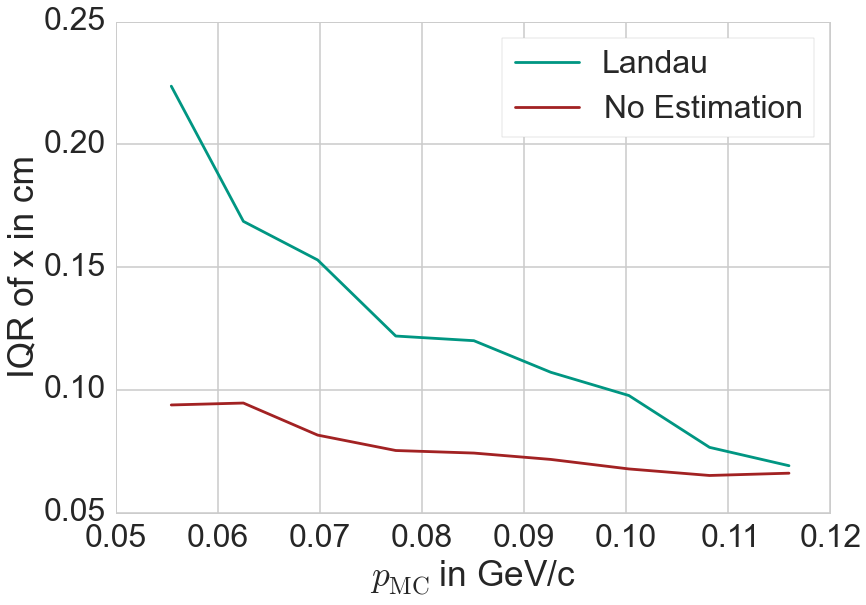
\includegraphics[width=0.48\linewidth]{figures/vxd/perigee_x.png}
  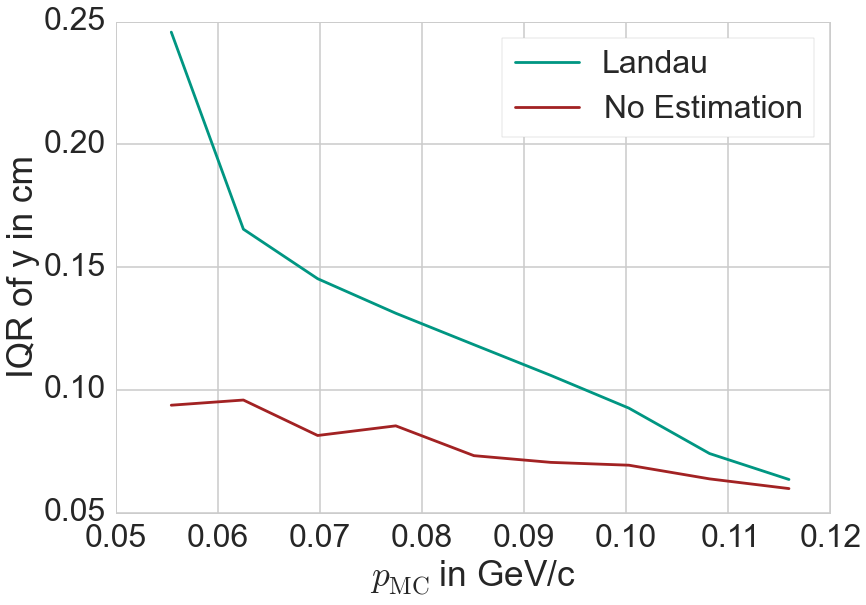
\includegraphics[width=0.48\linewidth]{figures/vxd/perigee_y.png}
  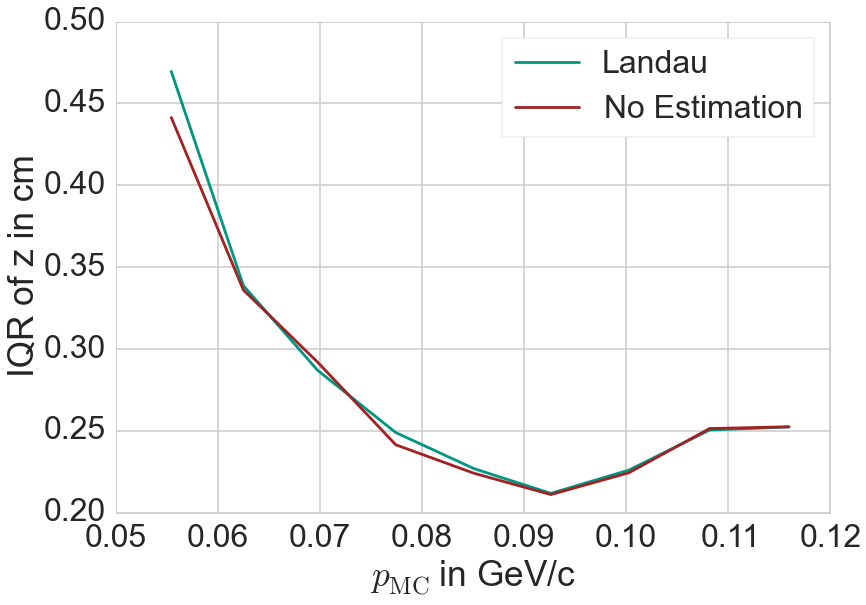
\includegraphics[width=0.48\linewidth]{figures/vxd/perigee_z.png}
  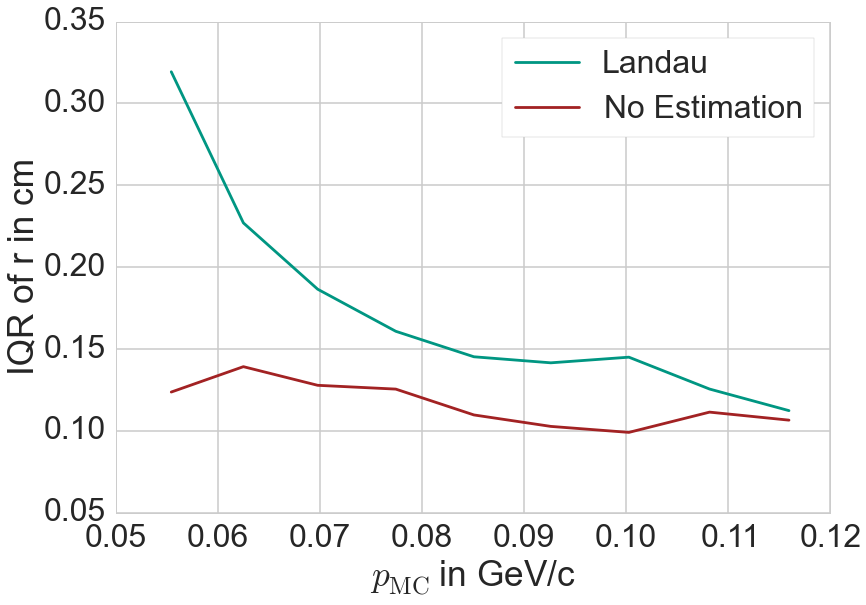
\includegraphics[width=0.48\linewidth]{figures/vxd/perigee_r.png}
  \caption[Perigee position with and without the momentum estimation.]{The IQR of the position at the perigee resulting from the helix fit with and without the momentum estimation. As the MC position is exactly zero, a residuum can not be calculated properly. The value of $r$ is calculated using $r=\sqrt{x^2 + y^2}$}
  \label{fig-position}
\end{figure}

% the pull distribution of the momentum and the three position resolutions is calculated and shown in figure \ref{fig-pull}. \todo{Beschreibung}

% \begin{figure}
%   \centering
%   \includegraphics[width=0.48\linewidth]{figures/vxd/pullMomentum.pdf}
%   \includegraphics[width=0.48\linewidth]{figures/vxd/pullPositionX.pdf}

%   \includegraphics[width=0.48\linewidth]{figures/vxd/pullPositionY.pdf}
%   \includegraphics[width=0.48\linewidth]{figures/vxd/pullPositionZ.pdf}
%   \todo{picture}
%   \caption[Pull distributions for the total momentum and the three coordinates of the perigee.]{Pull distributions for the total momentum and the three coordinates of the perigee. TODO: Beschreibung}
%   \label{fig-pull}
% \end{figure}

The next analysis is concerning the errors included into the momentum measurement. As the error is included as a fixed value for all momenta, it is not expected to be correct. Nevertheless the p-value of the whole track fit is presented in figure \ref{fig-p-values} with and without the VXD momentum estimation again with CDC and VXD tracks merged. The error introduced in the new measurement seems to be underestimated which causes the p-value to shift to smaller values. This can be caused by the fixed value of the error for all momenta (which is definitely wrong as the residuum distribution behaves differently for different momenta as seen in figure \ref{fig-results-fit}). Another reason is the distribution of \dedx for a fixed momenta - a landau distribution - which has a long tail towards higher energy losses and can therefore not be described well by a gaussian distribution (which must be used to calculate the error in genfit). Here is probably much room for improvement in further developments.

\begin{figure}
  \centering
  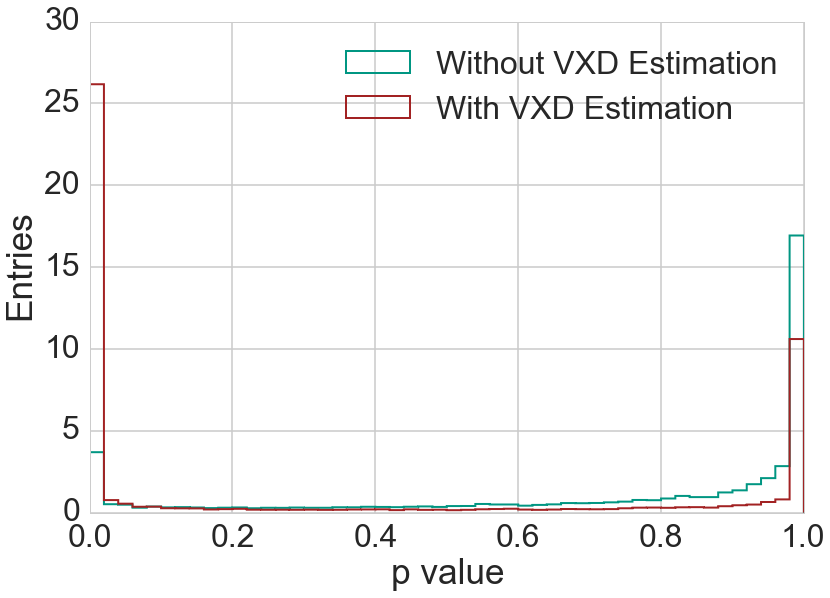
\includegraphics[width=0.7\linewidth]{figures/vxd/pValue.png}
  \caption[P-values of the whole track fit]{P-values of the whole track fit with and without the VXD momentum estimation for merged CDC and VXD tracks with the landau fit function and path lengths calculated with the current fit state. The p-value is much lower with the VXD momentum estimation indicating underestimated errors introduced in the fit.}
  \label{fig-p-values}
\end{figure}


\section{Conclusion and further possibilities}

By introducing a new measurement type into the fit of VXD tracks using a prefitted momentum estimator function and the \dedx value, the resolution of the momentum after the fit could be increased for low momenta tracks. The handling of the error of this measurement and the correlations to the other coordinates (especially the local position coordinates) must be further analyzed to enhance the position information and the p-values again. Also a better handling of the decision when to apply the momentum estimation should be included. The \texttt{MeasurementCreator} and the measurement type of the VXD momentum estimation should be constructed in such a way to handle these improvements.

A different approach was used in other experiments \cite{sergey}: the fitting algorithm calculates the energy loss in every sensor when handling the material effects in every fit step. This energy loss can be compared to the one measured by the sensors and the fit parameters can be corrected. This method has the benefit of not needing a momentum estimator function for transforming the \dedx value to a momentum estimation as it uses the raw \dedx information. It also does not need to calculate the path length by using a helix parametrization but uses the step length in every fit step. The downside of this approach is, that it relies on a correctly calibrated measured energy loss in the sensor with which it can compare. Another disadvantage is that the energy loss measurement can not be handled in the same way as the other measurements and there is not possibility to downweight it in the DAF algorithm or include the correlation to the coordinate measurements. When it comes to the underestimated error because of the landau tail and the condition when to include this momentum estimation, this approach shares the same problems as the here presented.

